%_______________________________________________________________________________
%class
%_______________________________________________________________________________
%\documentclass[a4paper,11pt,onecolumn,final,german,openbib]{scrbook}
\documentclass[a4paper,11pt,oneside,final,english,toc=bib,draft]{scrbook}

% fonts

\usepackage{fontspec}
\setmainfont{Libre Baskerville} % Libre Baskerville - Palatino Linotype - Constantia
\setsansfont{Helvetica} % Arial
\setmonofont{Consolas} % Hack

\usepackage[OT1]{eulervm}
% \usepackage{mathdesign}

%_______________________________________________________________________________
% page borders
%_______________________________________________________________________________
\addtolength{\headheight}{2cm}
%\addtolength{\topmargin}{2cm}
\setlength{\oddsidemargin}{1.0cm}
\setlength{\evensidemargin}{0.5cm}
\setlength{\textwidth}{14.3cm}
\setlength{\parindent}{0mm}

%_______________________________________________________________________________
% packages
%_______________________________________________________________________________
% \usepackage{german}
\usepackage{babel}[uk-english]
% \usepackage{textcomp}
\usepackage{csquotes}

\usepackage{mathtools}
\usepackage{amssymb,amsfonts}
\usepackage{physics}
\usepackage[separate-uncertainty=true,per-mode=power,group-separator={,}]{siunitx} % ,per-mode=fraction 
% \usepackage[version=4]{mhchem}
% \usepackage{dsfont}
% \usepackage{slashed}

\usepackage{graphicx}
\usepackage{xcolor}
% \usepackage{subfigure}
\usepackage{float}
\usepackage{caption}
\usepackage{subcaption}
\usepackage{enumitem}

% \usepackage{url}
% \usepackage{enumerate}

\usepackage{booktabs}
% \usepackage{multirow}

% \usepackage{appendix}

\usepackage{todonotes}

\usepackage[style=ieee]{biblatex} % ,sorting=none style=h-physrev3 defernumbers=true
\bibliography{thesis}


\graphicspath{ {./images/} }

\usepackage[draft=false]{hyperref}
\hypersetup{
  colorlinks=true,
  linkcolor=blue,
  citecolor=teal
}

\captionsetup[figure]{labelfont=bf,format=plain,labelsep=newline} % ,labelsep=period ,margin=1cm
\captionsetup[table]{labelfont=bf,format=hang,labelsep=space} % ,labelsep=period ,margin=1cm ,labelsep=newline

\renewcommand{\arraystretch}{1.2}

\newcommand{\figwidth}{12cm}

\parindent10mm

% \makesavenoteenv{table}

\usepackage{mgscience}

%_______________________________________________________________________________
% bold fonts for headings
%_______________________________________________________________________________
\font\afont=cmssbx10 scaled \magstep5     % for the title
\font\bfont=cmssbx10 scaled \magstep4     % for chapter headings
\font\cfont=cmssbx10 scaled \magstep3
\font\dfont=cmssbx10 scaled \magstep2     % for section headings and author name
\font\efont=cmssbx10 scaled \magstephalf

%_______________________________________________________________________________
% index depth
%_______________________________________________________________________________
\setcounter{secnumdepth}{3}
\setcounter{tocdepth}{3}

%_______________________________________________________________________________
% new commands
%_______________________________________________________________________________
% \newcommand{\demi}{\frac{1}{2}}

%_______________________________________________________________________________
% renewed commands
%_______________________________________________________________________________
% \renewcommand{\topfraction}{1.}       % this is important for figure placement
% \renewcommand{\bottomfraction}{1.}
\makeatletter
\renewcommand\paragraph{\@startsection{paragraph}{4}{\z@}%
  {-3.25ex\@plus -1ex \@minus -.2ex}%
  {1.5ex \@plus .2ex}%
  {\normalfont\normalsize\bfseries}
}
\makeatother

%_______________________________________________________________________________
% special words, hyphenation
%_______________________________________________________________________________
% \hyphenation{Ba-che-lor-ar-beit}

\pagestyle{empty}
\pagestyle{headings}
%for changing the style on a specific page use \thispagestyle{e.g., empty}

%_______________________________________________________________________________
%_______________________________________________________________________________
\begin{document}
\pagenumbering{roman}

%_______________________________________________________________________________
\begin{titlepage}
  \vspace*{6mm}
  \begin{center}
     {\afont Comparison of 3-dimensional chromatin structures based on single cell Hi-C data}
     \\[3.5cm]
     {\large von}
     \\[3.5cm]
     {\dfont Moritz Gmeiner}
     \\[1.5cm]
     {\dfont Supervisor: PD Dr. Peter Virnau}
     \\[2cm]
     % {\large Bachelorarbeit in Physik \/\\
     %    vorgelegt dem Fachbereich Physik, Mathematik und Informatik (FB 08) \/\\
     %    der Johannes Gutenberg-Universität Mainz \/\\
     %    am 1. April 2012}
     {\large Bachelor Thesis in Physics \/\\
        presented to the faculty physics, mathematics, and computer science (FB 08) \/\\
        of the Johannes Gutenberg University Mainz \/\\
        \today}
   \end{center}
   \vfill
   1. Reviewer: PD Dr. Peter Virnau \\	
   2. Reviewer: Prof. Dr. Friederike Schmid \\
   \vfill
\end{titlepage}

\thispagestyle{empty}
Ich versichere, dass ich die Arbeit selbstständig verfasst und keine 
anderen als die angegebenen Quellen und Hilfsmittel benutzt sowie 
Zitate kenntlich gemacht habe.
\\
\\[3.5cm] 
Mainz, den \today
\vfill
\noindent 
Moritz Gmeiner\\
KOMET\\
Institut für Physik\\
Staudingerweg 7\\
Johannes Gutenberg-Universität
D-55099 Mainz\\
{ \texttt{mgmeiner@students.uni-mainz.de} }

%_______________________________________________________________________________
% \renewcommand\contentsname{Inhaltsverzeichnis}
% \renewcommand\figurename{Abbildung}
% \renewcommand\tablename{Tabelle}

\tableofcontents
\clearpage

\mainmatter
\sloppy

%_______________________________________________________________________________
% \include{...}
\chapter{Introduction} % (fold)
\label{cha:introduction}

{\em Dieses Dokument richtet sich an Studierende am Fachbereich 08 im 
Studiengang Bachelor of Science (Physik). Sie finden hier Beispiele 
für eine mögliche Gliederung Ihrer Arbeit und Hinweise zur 
Strukturierung des Inhalts. Selbstverständlich sollen Sie diese 
Gliederung nach den Gegebenheiten Ihrer Bachelorarbeit anpassen. 
Besprechen Sie rechtzeitig mit Ihrem Betreuer, ob Ihr Entwurf sinnvoll 
ist. Holen Sie sich auch Anregungen zur Gestaltung von Abschlussarbeiten 
aus der Literatur (siehe z.\ B.\ \verb|\cite{EbelBliefert}|).}

\medskip

\textcolor{orange}{In der Einleitung Ihrer Bachelorarbeit sollte das Thema der Arbeit 
möglichst allgemeinverständlich eingeführt werden. Gehen Sie 
dabei auch auf das weitere Umfeld der Arbeit ein und erläutern Sie, 
warum Aufgabenstellung und Herangehensweise interessant sind. Auch 
die weitere Gliederung kann angesprochen werden, um dem Leser einen 
ersten überblick über den nachfolgenden Text zu geben.}

\bigskip

The goal of this thesis is to explore the chromatin structure of DNA in the nucleus further, based mainly on previous the research in \cite{wettermann_minimal_2020}.

DNA is in the nucleus. Structure of DNA is important. DNA structure is lost during mitosis and has to reestablished later. Structure is important for transcription and differentiation.

\bigskip

\section{Mathematical Tools} % (fold)
\label{sec:mathematical_tools}

\subsection{RMSD} % (fold)
\label{sec:rmsd}

The root-mean-square deviation (RMSD) is a mathematical tools for comparing how similar two ordered sets of 3-dimensional points of equal length are and is given for the two sets \( \set{x_i} \) and \( \set{y_i} \) by the formula

\[
  \text{RMSD} = \sqrt{ \frac{n} \sum_i \norm{x_i - y_i}^2 }
\]



% section rmsd (end)

% section mathematical_tools (end)



%_______________________________________________________________________________
% \chapter{Main Part}

% Die typische Gliederung einer Bachelorarbeit könnte so aussehen, 
% wie im folgenden dargestellt. 
% \medskip

% Verwenden Sie aussagekräftige Kapitelüberschriften, also zum 
% Beispiel {\em Aufbau eines Teilchenbeschleunigers} statt 
% {\em Versuchsaufbau}.


% chapter introduction (end)

%_______________________________________________________________________________


%!TEX root = ../thesis

\chapter{Simulation} % (fold)
\label{cha:simulation}

\section{Model and Simulation Protocol} % (fold)
\label{sec:model_and_simulation_protocol}

The simulation protocol for the entire genome simulations was mostly carried over from (Wettermann et al.\cite{wettermann_minimal_2020}). Additionally simulations of single chromosomes were carried out; the protocol for these simulations is identical to that of the entire genome, except only the beads of the chromosome in question were modelled. The simulation is a molecular dynamics simulation using the HOOMD-blue\cite{anderson_hoomd-blue_2020} toolkit. It utilises a Langevin integrator (\verb|hoomd.md.integrate.langevin|) with a timestep of \(dt=0.001\), a temperature of \(kT = 1.0\), and a drag coefficient of \(\gamma = 1.0\). The neighbour list is a BVH tree neighbour list \cite{howard_efficient_2016} \cite{howard_quantized_2019} that was originally chosen as it scales
with particle number as opposed to the system volume\cite{wettermann_minimal_2020}.

Each chromosome is modelled as beads on a string, where each bead represents a bin of \(\SI{100000}{bp}\). This is the same resolution as was chosen in (Wettermann et al.\cite{wettermann_minimal_2020}) and represents a compromise between the resolution of the simulation result and the quality of the contact data that is available: a higher resolution, i.e. a smaller bin size of for example \(\SI{40000}{bp}\), would increase the resolution of the simulated structure and enable us to see smaller structures, but at the same time would spread the fixed number of contacts across a higher number of beads. This would make in particular the effect of having captured only a fraction of all possible contacts in the cell using Hi-C more prominent, which is estimated to be around \(5\%\) for each cell as seen in Table~\ref{tab:contact_capture}. Vice versa, decreasing the bin size would help mitigate the partial capture of contacts, but limit the spatial resolution of the simulated structure. With this chosen resolution of \(\SI{100000}{bp}\) per bin the genome is represented by 20 chains varying in length between 500 and 2,000 beads each (the exact lengths for each chromosome can be found in Table~\ref{tab:chrom_lengths}), or 25,714 beads in total. This does not represent the entirety of the mouse genome, whose length is approximately \(\SI{2632}{Mbp}\)\footnote{Mouse Genome Assembly GRCm39 from \url{https://www.ncbi.nlm.nih.gov/grc/mouse/data}, visited on 26.02.2022}, or 26,321 beads at a resolution of \(\SI{100000}{bp}\) per bead. The reason for this difference is that beads at the boundary of a chromosome that had no contact in any of the eight cells were dropped from the simulation, since their impact was assumed to be only negligible. Boundary beads that had contacts in some cells but not others were kept in the simulation of all cells in order to keep the simulation data consistent across cells.

The model is based on a generic bead-spring polymer model in which three kinds of bonds are defined. The first two kinds of bonds are harmonic bonds between two beads of the general form

\[
  V(r) = \frac{2} \kappa \left( r - r_0 \right)^2
\]

where \(\kappa\) is the force constant determining the stiffness of the bond, which is fixed at \(\kappa = 2000\) for all harmonic bonds, and \(r_0\) is the preferred bond distance. The first kind of harmonic bonds are the backbone bonds connecting adjacent beads in each chromosome; for these bonds the preferred distance is set to \(r_0 = 1.0 \). The other kind of harmonic bonds in the simulation are the predefined contacts derived from the Hi-C data set from (Stevens et al.\cite{stevens_3d_2017}). Here the preferred bond distance is set a little larger compared to the backbone at \(r_0 = 1.5\) in accordance with (Wettermann et al.\cite{wettermann_minimal_2020}).

The third kind of bond is a Gaussian pair potential of the form

\[
  V(r) = \begin{cases}
    \epsilon \exp \left[ - \frac{2} \left( \frac{r}{\sigma} \right)^2 \right] & r < r_\text{cut} \\
    0 & r \geq r_\text{cut}
  \end{cases}
\]

between all beads in the simulation designed to push all non-bonded beads away from each other. This potential is used in 2 forms in different parts of the simulation: a full form with \(\sigma = 1.0\) and \(r_\text{cut} = 3.5\) and a reduced form with \(\sigma = 0.1\) and \(r_\text{cut} = 0.4\); in both cases \(\epsilon = 100\). On one hand, this mimics the fact that at physiological conditions DNA molecules are negatively charged and thus repels each other. On the other hand it represents an excluded volume potential that pushes all beads away from each other, which is  quite significant for the emergence of chromosomal territories\cite{wettermann_minimal_2020}. An overview of all the potentials in the simulation can be seen in Figure~\ref{fig:potentials}.

\begin{figure}[ht]
\centering
  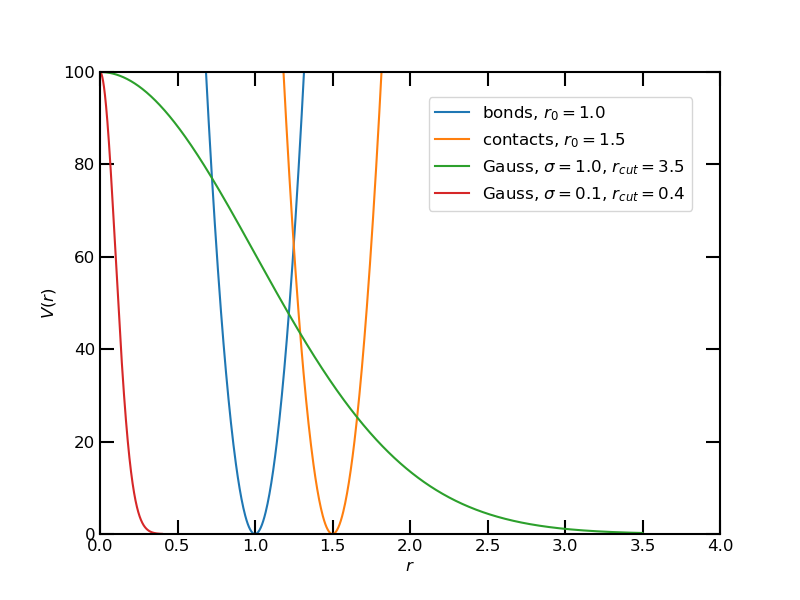
\includegraphics[width=\figwidth]{potentials.png}
  \caption{Potentials used in the simulation. Bonds and contacts are harmonic potentials of the form \(V(r) = 1000 (r - r_0)^2\), with bonds having an \(r_0\) of 1.0 and contacts having an \(r_0\) of 1.5. Gauss potentials are of the form \(V(r) = 100 \exp\left[- \frac{2} \left( \frac{r}{\sigma} \right)^2 \right]\) for \(r\) smaller than \(r_\text{cut}\) and \(0\) for \(r\) greater than the cutoff value \(r_\text{cut}\).}
  \label{fig:potentials}
\end{figure}

The system is initialised by distributing all the beads randomly throughout the simulation box (uniform distribution, using \verb|numpy.uniform.random|\cite{harris_array_2020}). The bonds are set and the simulation is repeatedly cycled through the following steps:

\begin{itemize}[label=\(\bullet\)]
  \item 80,000 time steps with no excluded volume potential
  \item 50,000 time steps with reduced volume potential
  \item 50,000 time steps with full excluded volume potential
\end{itemize}

Bonds and contacts are active at all of those steps. After each cycle the current state is saved to a gsd trajectory file. These saved states will be referred to in the following as \textbf{frames}. Frames whose trajectories are similar are said to have the same \textbf{configuration}. These steps were repeated in each simulation for a total of 105 cycles. The first few cycles have to be discarded as the system takes some time to find its ground state, although certain problems can arise here that will be discussed later in \ref{sec:problems_with_the_simulation}.

% section model_and_simulation_protocol (end)

\section{Simulation results} % (fold)
\label{sec:simulation_results}

Each simulation yields 105 sequential frames, i.e. the simulation state is not reset after each simulation cycle, but instead the final state of the last cycle is the initial state of the next cycle. This has the advantage of giving the system time to tune in, but also the disadvantage of the possibility that certain end configurations will never be reached in a particular simulation run after it has tuned in to a different locally minimal configuration. The potential energies of each frame for the simulation run of cell 2 can be seen in Figure~\ref{fig:potential_energy_cell2}. The first two frames show a potential energy significantly larger than the later ones, then the system quickly converges to a potential energy of about \(\num{7950000}\) and shows only small deviations of less than \(1 \%\) of the mean. Thus both the length of the settling period and the potential energy of the ground configuration match (Wettermann et al.\cite{wettermann_minimal_2020}) extremely well. To minimise the effect of the settling period the first 5 frames of each simulation run will generally be excluded in all subsequent analyses where the data is combined over all frames such as averages or standard deviations.

Furthermore, Figure~\ref{fig:distance_pdf_cell2} shows the distance distribution of the bonds and predetermined contacts combined across all frames of the simulation of cell 2. The results are again very similar to (Wettermann et al.\cite{wettermann_minimal_2020}), with both peaks and means shifted slightly to the right of the respective preferred bond length of \(1.0\) and \(1.5\). The \(99.73\)th quartile is at \(1.71\) for bonds and \(2.42\) for contacts, showing that a substantial portion of the bonds and predetermined contacts are enforced reasonably well.

\begin{figure}[ht]
\centering
  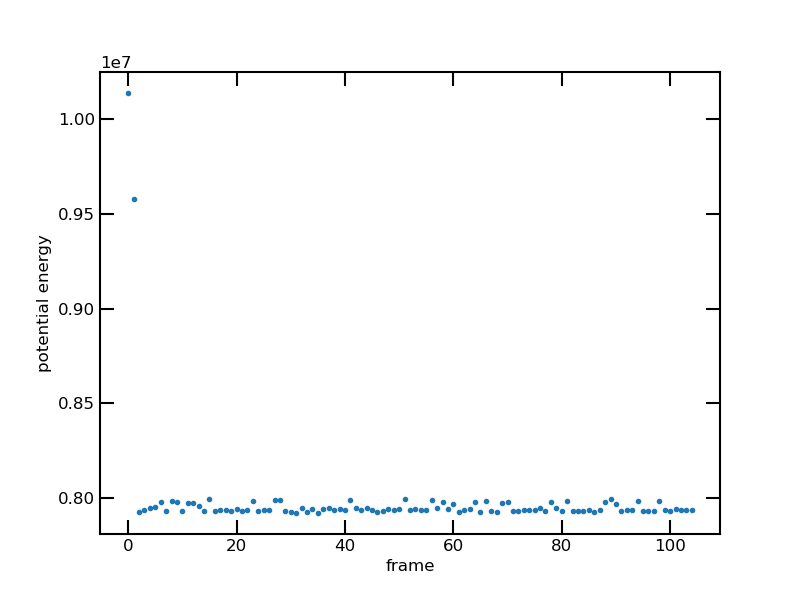
\includegraphics[width=12cm]{potential_energy_cell2.png}
  \caption{Potential energy of each frame in the simulation of cell 2.}
  \label{fig:potential_energy_cell2}
\end{figure}

\begin{figure}[ht]
\centering
  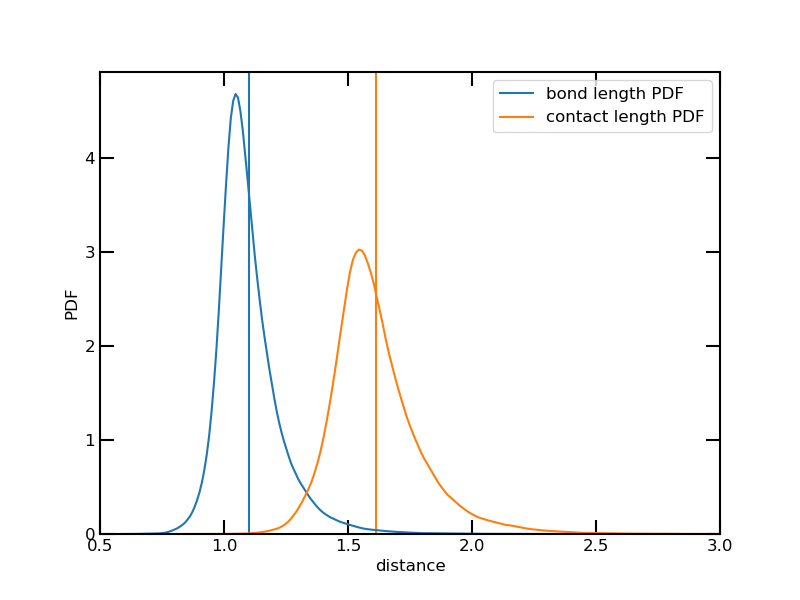
\includegraphics[width=12cm]{distance_pdf_cell2.png}
  \caption{Distance distributions for bonds and predetermined contacts over all frames in the simulation of cell 2 with the means marked by a vertical line. The mean of the bond distances is at \(\num{1.10}\) and the mean of the contact distances is at \(\num{1.61}\).}
  \label{fig:distance_pdf_cell2}
\end{figure}

For the other cells the situation is generally similar, except for cell 1 and cell 5, which will be discussed more in-depth in \ref{sec:problems_with_the_simulation}. The coefficients of variation, i.e. the standard deviations divided by the means, of potential energies are between \(0.3\%\) and \(1.8\%\), showing the minimum energy configuration to be quite stable in these cells. Also neither bonds nor contacts are overly overstretched in any cells, including cell 1 and cell 5. A complete overview of potential energy coefficients of variation and means and \(99.73\)th percentiles for bonds and predefined contacts can be found in Table~\ref{tab:simulation_pe_dists}.

Renderings of all simulated cells can be seen in Appendix~\ref{cha:renderings_of_simuated_cells}. A few things can be notes from these images visually. First, most simulated genomes have a quite regular, spherical shape, but in particular cell 3, cell 8, and the higher energy configuration of cell 5 (which will be discussed in more detail in \ref{sec:problems_with_the_simulation}) show clear differences from this. Cell 3 and cell 8 have a more elongated, bean-like shape, as can be seen in Figure~\ref{img:cell3_frame104_scene1} for cell 3 and in Figure~\ref{img:cell8_frame104_scene2} for cell 8. The higher energy configuration of cell 5 on the other hand has a more obloid, donut-like shape. Also notable is the fact that cell 6 and cell 7 are hollow as can be seen for example in Figure~\ref{img:cell6_frame104_scene1} for cell 6 and Figure~\ref{img:cell7_frame104_scene1} for cell 7. More renderings of all simulated cells can be seen in Appendix \ref{cha:renderings_of_simuated_cells}.

% section simulation_results (end)

\section{Problems with the simulation} % (fold)
\label{sec:problems_with_the_simulation}

While the simulations of most cells quickly reached a stable ground state configuration, the simulations of cell 1 and of cell 5 showed significant deviation from the expected results, warranting further investigation.

\subsection{Cell 1} % (fold)
\label{sub:cell_1}

In cell 1, a ground state is reached very quickly, but this ground state is very unstable, as indicated by the comparably high coefficient of variation of the potential energy of 8.51\% in Table~\ref{tab:simulation_pe_dists} and seen in Figure~\ref{fig:potential_energy_cell1}. The RMSDs of all frames with respect to the last frame as seen in Figure~\ref{fig:rmsd_cell1} shows that some of these frames have rather similar configurations while others are very different. One hypothesis would be that some frames represent a ground state configuration while others are higher energy states. This can be tested by selecting for all frames with low energy, defined by being below some cutoff energy, and checking how the RMSDs for those low-energy frames behaves. A cutoff energy of \(\num{1.495e7}\), visually displayed in Figure~\ref{fig:potential_energy_cell1} as the orange line, was chosen as it captures most of the frames that can be identified visually as being low energy, while excluding all that deviate strongly from this energy baseline. This selects a total of 52 frames, which have been marked in Figure~\ref{fig:rmsd_cell1} by red dot. As can be seen very clearly, these low energy frames do in fact have a low RMSD of \(\num{1.00(1)}\) with respect to the last frame. This confirms that while it is very unstable, this simulation of cell 1 does in fact have a ground state configuration, and it can be filtered for by selecting for those frames with a low energy. To check if this ground state instability is an intrinsic property of the Hi-C contact data for cell 1 or merely a random artefact of this particular simulation run, cell 1 was simulated two more times. The potential energies for those repeated simulations can be seen in Figure~\ref{fig:potential_energy_cell1_1} and Figure~\ref{fig:potential_energy_cell1_2} in the appendix and clearly show the same pattern of instability, leading to the conclusion that this instability is in fact a consequence of the predetermined contacts for cell 1.

\begin{figure}[ht]
\centering
  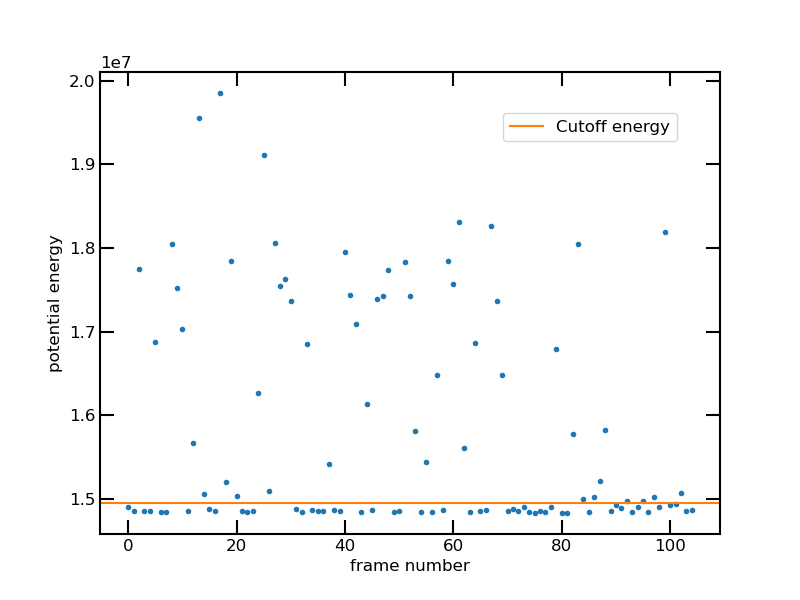
\includegraphics[width=10.5cm]{potential_energy_cell1.png}
  \caption{Potential energies of all frames in the simulation of cell 1. Cutoff energy is set at \(\num{1.495e7}\), with all frames lower than this threshold being defined as \enquote{low-energy frames}.}
  \label{fig:potential_energy_cell1}
\end{figure}

\begin{figure}[ht]
\centering
  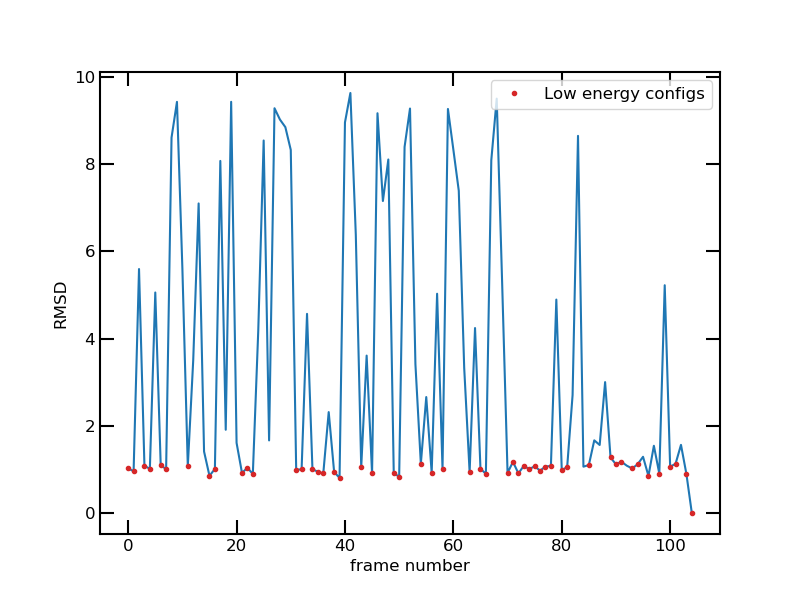
\includegraphics[width=10.5cm]{rmsd_cell1.png}
  \caption{RMSDs of cell 1 with respect to last frame. Low-energy frames, as defined in Figure~\ref{fig:potential_energy_cell1} to be frames with a potential energy lower than \(\num{1.495e7}\), have their RMSD marked by a red dot.}
  \label{fig:rmsd_cell1}
\end{figure}

% subsection cell_1 (end)

\FloatBarrier

\subsection{Cell 5} % (fold)
\label{sub:cell_5}

Figure~\ref{fig:potential_energy_cell5_all} shows the potential energies of all frames in the simulation of cell 5 in blue. As can be seen, after the zeroth frame, which is of higher energy as is typical for the transient phase, the potential energy drops to and stabilises around a value of \(\num{9.805(43)e6}\) for frames 1 through 38. But then for frame 39 and the following ones until the end of the simulation, the energy drops down again to a significantly lower value of \(\num{8.220(8)e6}\). As seen in Figure~\ref{fig:potential_energy_cell5_all}, this is a reduction in both the potential energy itself as well as the deviation in potential energy, from a coefficient of variation of \(0.5 \%\) down to \(0.1 \%\), signifying that the second configuration is both energetically more favourable as well as very stable. The fact that the first configuration was held for 38 frames though means that the existance of semi-stable configurations apart from the ground state configuration is possible. To examine this effect further, cell 5 was simulated 2 more times. The resulting potential energies, together with the potential energies of the first simulation, can be seen in Figure~\ref{fig:potential_energy_cell5_all}. Clearly the second and third simulation run show the same pattern that most other cells exhibit: the first one or two frames have a higher potential energy, and then it drops into a stable ground state configuration where it remains for the rest of the simulation. The very similar potential energies of the ground state configurations in all three simulations suggests that these ground state configurations are in fact the same across all simulations. An analysis of the RMSDs of each frame in all three simulations from the last frame of the first simulation can be seen in Figure~\ref{fig:rmsd_cell5_all} and clearly confirms that the ground states of all three simulations are in fact the same one. This means that while the simulation of cell 5 does have a single stable ground state configuration, it also has a semi-stable configuration that arises in some, but not all simulation runs.

% \begin{figure}[ht]
% \centering
%   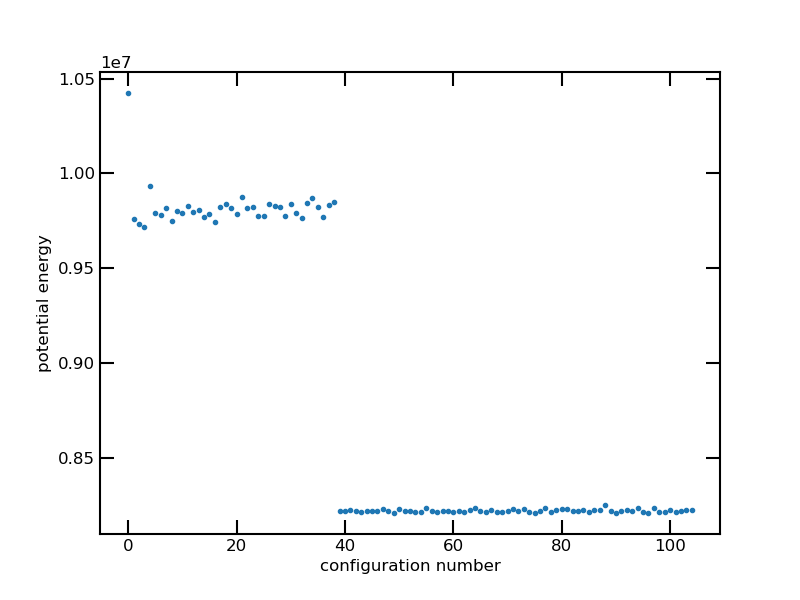
\includegraphics[width=\figwidth]{potential_energy_cell5.png}
%   \caption{Potential energies of all frames in the (first) simulation of cell 5.}
%   \label{fig:potential_energy_cell5}
% \end{figure}

\begin{figure}[ht]
\centering
  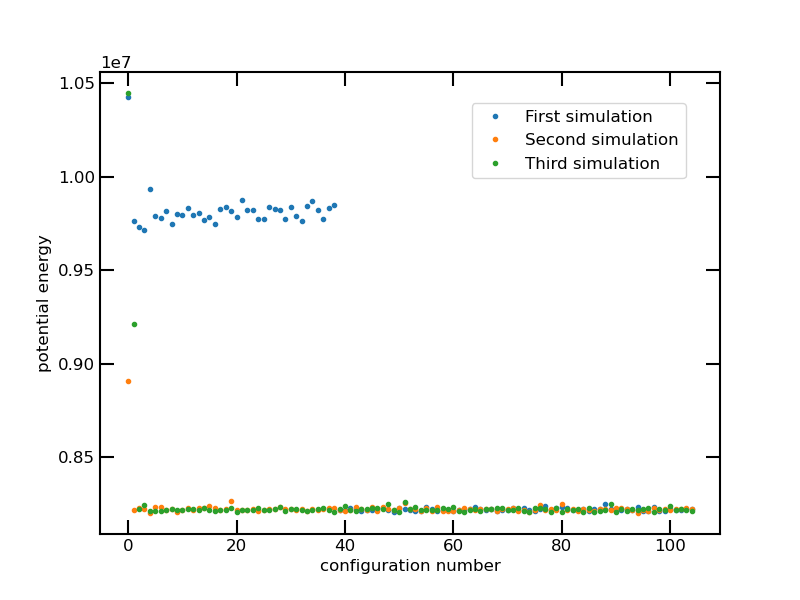
\includegraphics[width=\figwidth]{potential_energy_cell5_all.png}
  \caption{Potential energies of all frames in all three simulations of cell 5.}
  \label{fig:potential_energy_cell5_all}
\end{figure}

\begin{figure}[ht]
\centering
  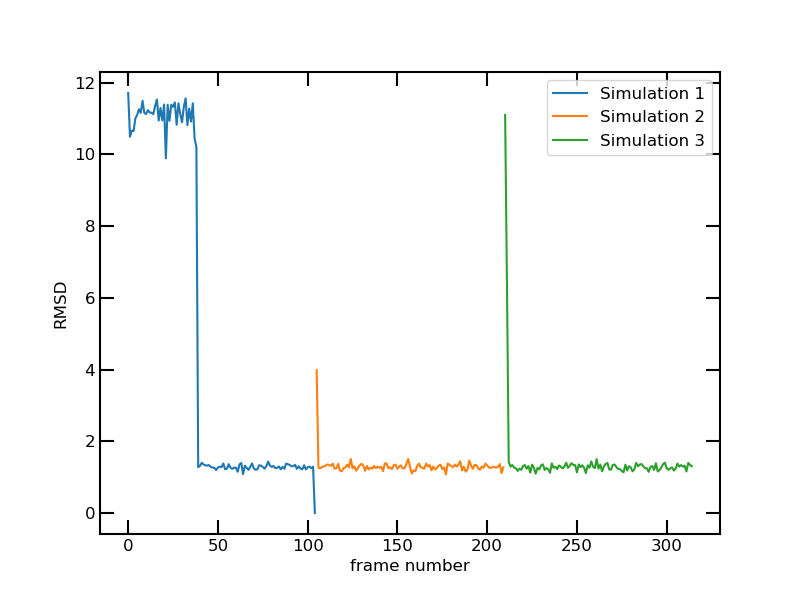
\includegraphics[width=\figwidth]{rmsd_cell5_all.png}
  \caption{RMSD of all three simulations of cell 5 with respect to the last frame of the first simulation.}
  \label{fig:rmsd_cell5_all}
\end{figure}

% subsection cell_5 (end)

% section problems_with_the_simulation (end)


% chapter simulation (end)


%_______________________________________________________________________________



\chapter{Comparison of Cells} % (fold)
\label{cha:comparison_of_cells}

\section{Definition of SCC} % (fold)
\label{sec:definition_of_scc}

HiCRep is a mathematical tool introduced in \cite{yang_hicrep_2017} for the explicit goal of comparing Hi-C data sets. It takes as input the contact matrices of two Hi-C data sets and outputs a correlation coefficient, that is a number between \(-1\) and \(1\), with higher numbers signifying a stronger similarity between the data sets and vice versa. This is done in a two-step process: first both contact matrices are smoothed to counter binning-associated problems and then a stratuma djusted correlation coefficient (SCC) is calculated between these smoothed contact matrices. The exact procedure will be explained in the following section

\subsection{Smoothing} % (fold)
\label{subsec:smoothing}

Both contact maps are first smoothed using a uniform filter of width \(2h+1\) for a chosen smoothing parameter \(h \geq 0\). This helps compensating a lack of coverage, that is the fact that not all actual contacts are contained in the contact matrices, something that is common for Hi-C data. Mathematically this filter is defined as

\[
  X_{ij} = \frac{ \sum_{k=i-h}^{i+h} \sum_{l=j-h}^{j+h} C_{kl} }{ 2h+1 }
\]

where \(C\) is the \(n \times n\) contact matrix and \(X\) is the \(n \times n\) smoothed matrix. \(C_{ij}\) is defined to be 0 for either \(i\) or \(j\) not in \(1 \dots n\).

The uniform filter might seem like an unusual choice compared to other more sophisticated filters, but has the great advantage of having the representation \( X = L \cdot C \cdot R \), where \(X\) is the smoothed matrix, \(C\) is the contact matrix, and \(L\) and \(R\) are upper and lower trigangular matrices respectively. This comes in handy especially when using sparse representations of \(C\) and \(X\), which is very much recommended since contact matrices generally can be quite large and are largely empty.

\(h\) is a parameter for the SCC algorithm and thus has to be chosen appropriately. The HiCRep package includes a function called \verb|htrain| (\verb|h_train| in the HiCRep.py python package) that tries to estimate an appropriate h-value heuristically. For our resolution of \(\SI{100}{kbp}\) an example value of \( h = 3 \) is given in the original HiCRep paper, which should be kept in mind as a refence later when trying to choose an h-value for our own data.

% subsection smoothing (end)

\subsection{SCC} % (fold)
\label{subsec:scc}

The stratum adjusted correlation coefficient aims to be a measure of correlation between two random variables \(X\) and \(Y\), stratified by a third variable into \(K\) strata \(X_1, \dots, X_K\) and \(Y_1, \dots, Y_K\) respectively. In each stratum we have the stratified random variables \((X_k, Y_k)\) with \(N_k\) observations \( (x_{k,1}, y_{k,1}), \dots, (x_{k,N_k}, y_{k,N_k}) \) each. The pearson correlation coefficient between \(X\) and \(Y\) for the k-th stratum is given by

\[
  \rho_k = \frac{ \mathrm{Cov}(X_k,Y_k) }{ \sqrt{ \mathrm{Var}(X_k) \mathrm{Var}(Y_k)} } = \frac{ \sum_{i=1}^{N_k} (x_{k,i} - \overbar{x}_k) (y_{k,i} - \overbar{y}_k) }{ \sqrt{ \sum_{i=1}^{N_k} x_{k,i} - \overbar{x}_k } \sqrt{ \sum_{i=1}^{N_k} y_{k,i} - \overbar{y}_k } }
\]

The SCC is the weighted average of the pearson correlation coefficients

\[
  \rho_s = \sum_{k=1}^{K} w_k \rho_k
\]

where the weights \(w_k\) are

\[
  w_k = \sqrt{ \mathrm{Var}\left( \frac{ \mathrm{Rank}(X_k) }{ N_k } \right) \mathrm{Var}\left( \frac{ \mathrm{Rank}(Y_k) }{ N_k } \right) }
\]

with \( \mathrm{Rank}(X_k) \) and \( \mathrm{Rank}(Y_k) \) being the ranked variables\footnote{\url{https://en.wikipedia.org/wiki/Ranking\#Ranking_in_statistics}}. For a thorough derivation of the SCC see the original HiCRep paper\cite{yang_hicrep_2017}, Section \enquote{Derivation of stratum-adjusted correlation coefficient (SCC)}.

% section definition_of_scc (end)

\section{SCC between cells} % (fold)
\label{sec:scc_between_cells}

The SCC for the Hi-C data of all cells can be seen in Table~\ref{tab:scc_hic}. It is immediately very clear that all SCC values except for those of a cell with itself are very low, especially compared to the values of \(0.7\) to \(1.0\) obtained in \cite{yang_hicrep_2017} for hESC (human embryonic stem cells) and IMR90 (human lung fibroblast cells) cell lines (see Figure~3A). This might very likely be related to the fact that each Hi-C data set captured only about \(5\%\) of all contacts, as detailed in Table~\ref{tab:contact_capture}, but regardless of the reasons, it sets the expectations for comparability between the cells quite low. The SCC for the simulated contact matrices can be seen in Table~\ref{tab:scc_sim} and, as expected, are similarly low.

\begin{table}[ht]
\centering
  \sisetup{ table-alignment-mode=none }
  \caption{\textcolor{red}{SCC between HiC contact matrices}}
  \label{tab:scc_hic}
  \begin{tabular}{S | S S S S S S S S}
   & {Cell 1} & {Cell 2} & {Cell 3} & {Cell 4} & {Cell 5} & {Cell 6} & {Cell 7} & {Cell 8} \\
  \midrule
    {Cell 1} &  {-}  & 0.132 & 0.093 & 0.116 & 0.128 & 0.105 & 0.136 & 0.092 \\
    {Cell 2} & 0.132 &  {-}  & 0.098 & 0.104 & 0.147 & 0.116 & 0.150 & 0.138 \\
    {Cell 3} & 0.093 & 0.098 &  {-}  & 0.062 & 0.104 & 0.093 & 0.101 & 0.092 \\
    {Cell 4} & 0.116 & 0.104 & 0.062 &  {-}  & 0.108 & 0.101 & 0.123 & 0.077 \\
    {Cell 5} & 0.128 & 0.147 & 0.104 & 0.108 &  {-}  & 0.121 & 0.148 & 0.123 \\
    {Cell 6} & 0.105 & 0.116 & 0.093 & 0.101 & 0.121 &  {-}  & 0.145 & 0.097 \\
    {Cell 7} & 0.136 & 0.150 & 0.101 & 0.123 & 0.148 & 0.145 &  {-}  & 0.116 \\
    {Cell 8} & 0.092 & 0.138 & 0.092 & 0.077 & 0.123 & 0.097 & 0.116 &  {-}  \\
  \end{tabular}
\end{table}

\begin{table}[ht]
\centering
  \sisetup{ table-alignment-mode=none }
  \caption{\textcolor{red}{SCC between simulated contact matrices}}
  \label{tab:scc_sim}
  \begin{tabular}{S | S S S S S S S S}
   & {Cell 1} & {Cell 2} & {Cell 3} & {Cell 4} & {Cell 5} & {Cell 6} & {Cell 7} & {Cell 8} \\
  \midrule
    {Cell 1} &  {-}  & 0.171 & 0.149 & 0.114 & 0.173 & 0.141 & 0.178 & 0.104 \\
    {Cell 2} & 0.171 &  {-}  & 0.164 & 0.141 & 0.183 & 0.184 & 0.215 & 0.184 \\
    {Cell 3} & 0.149 & 0.164 &  {-}  & 0.109 & 0.161 & 0.124 & 0.145 & 0.122 \\
    {Cell 4} & 0.114 & 0.141 & 0.109 &  {-}  & 0.135 & 0.105 & 0.140 & 0.098 \\
    {Cell 5} & 0.173 & 0.183 & 0.161 & 0.135 &  {-}  & 0.148 & 0.194 & 0.143 \\
    {Cell 6} & 0.141 & 0.184 & 0.124 & 0.105 & 0.148 &  {-}  & 0.191 & 0.116 \\
    {Cell 7} & 0.178 & 0.215 & 0.145 & 0.140 & 0.194 & 0.191 &  {-}  & 0.157 \\
    {Cell 8} & 0.104 & 0.184 & 0.122 & 0.098 & 0.143 & 0.116 & 0.157 &  {-}  \\
  \end{tabular}
\end{table}

% section scc_between_cells (end)

% chapter comparison_of_cells (end)

\chapter{Individual Chromosomes} % (fold)
\label{cha:individual_chromosomes}

% chapter individual_chromosomes (end)

%_______________________________________________________________________________
\chapter{Conclusion} % (fold)
\label{cha:conclusion}

In der Zusammenfassung sollten Sie in knapper Form die Aufgabenstellung 
und die wichtigsten Ergebnisse rekapitulieren. Es ist für die 
Gutachter hilfreich, wenn Sie ausdrücklich beschreiben, worin 
Ihre eigenen Beiträge liegen. Scheuen Sie sich auch nicht davor 
auszusprechen, welche Untersuchungen durch die Zeitbegrenzung der 
Bachelorarbeit nicht möglich waren und nutzen Sie dies als 
überleitung zu einem Ausblick auf mögliche weitergehende 
Arbeiten an der Aufgabenstellung.

% chapter conclusion (end)

\printbibliography

%_______________________________________________________________________________
\appendix

% \chapter{Appendix}
\chapter{Tables and Figures} % (fold)
\label{cha:tables_and_figures}

\textcolor{orange}{In der Regel sind die in Tabellen und Abbildungen enthalten Informationen 
so wichtig, dass sie im Hauptteil der Arbeit erscheinen sollten. Unter 
Umständen sind aber ergänzende Tabellen und Abbildungen gut in einem 
Anhang aufgehoben. Wie im Hauptteil sollten Sie auch hier darauf achten, 
dass die in Tabellen und Figuren (siehe Abb.\ ref{Abb:1}) dargestellte 
Information im Text angesprochen wird und selbsterklärende Legenden}
vorhanden sind.

\medskip

\begin{table}[H]
\centering
  \caption{Number of beads in each chromosome in the simulation. Each bead represents \(\SI{100}{kbp}\)}
  \label{tab:chrom_lengths}
  \begin{tabular}{c c c c c c c c c c c}
   \toprule
    Chrom & 1 & 2 & 3 & 4 & 5 & 6 & 7 & 8 & 9 & 10 \\
    Length & 1924 & 1791 & 1570 & 1534 & 1488 & 1466 & 1424 & 1263 & 1215 & 1275 \\
  \midrule
    Chrom & 11 & 12 & 13 & 14 & 15 & 16 & 17 & 18 & 19 & X \\
    Length & 1189 & 1171 & 1174 & 1218 & 1010 & 952 & 919 & 876 & 584 & 1671 \\
  \bottomrule
  \end{tabular}
\end{table}

\begin{table}[ht]
\centering
  \caption{\textcolor{red}{MAKE CAPTION}}
  \label{tab:simulation_pe_dists}
  \sisetup{ table-alignment-mode=none }
  \begin{tabular}{S @{\phantom{abc}} S @{\phantom{abc}} S @{\phantom{abc}} S @{\phantom{abc}} S @{\phantom{abc}} S}
  \toprule
     & & \multicolumn{2}{c}{bonds} & \multicolumn{2}{c}{contacts} \\
    {Cell} & \parbox{3cm}{pot energy \\ \% deviation} & {mean} & \parbox{3cm}{99.73th \\ percentile} & {mean} & \parbox{3cm}{99.73th \\ percentile} \\
  \midrule
    1 & 8.51\% & 1.13 & 1.98 & 1.62 & 2.72 \\
    2 & 0.27\% & 1.10 & 1.71 & 1.61 & 2.42 \\
    3 & 0.67\% & 1.14 & 1.88 & 1.68 & 2.52 \\
    4 & 1.83\% & 1.14 & 2.08 & 1.61 & 2.46 \\
    5 & 8.63\% & 1.11 & 1.81 & 1.62 & 2.55 \\
    6 & 0.94\% & 1.16 & 2.07 & 1.61 & 2.38 \\
    7 & 0.29\% & 1.10 & 1.58 & 1.59 & 2.09 \\
    8 & 0.28\% & 1.08 & 1.56 & 1.60 & 2.25 \\
  \bottomrule
  \end{tabular}
\end{table}

\begin{table}[ht]
\centering
  \caption{caption}
  \label{tab:contact_capture}
  \sisetup{ table-alignment-mode=none }
  \begin{tabular}{S S S S}
  \toprule
    {Cell} & \parbox{3cm}{\centering contacts specified} & \parbox{3cm}{\centering contacts after simulation} & \parbox{3cm}{\centering \% of contacts specified} \\
  \midrule
    1 & 48962 & 932831 & 5.2\% \\
    2 & 32243 & 558981 & 5.8\% \\
    3 & 19112 & 602439 & 3.2\% \\
    4 & 35514 & 685314 & 5.2\% \\
    5 & 31180 & 592569 & 5.3\% \\
    6 & 32862 & 358721 & 4.8\% \\
    7 & 21126 & 358721 & 5.9\% \\
    8 & 17581 & 320656 & 5.5\% \\
  \bottomrule
  \end{tabular}
\end{table}

% chapter tables_and_figures (end)


\chapter{Renderings of Simuated Cells} % (fold)
\label{cha:renderings_of_simuated_cells}

\newcommand{\cellrenderingwidth}{8cm}
\newcommand{\cellrenderingheight}{8cm}

All renderings rendered using VMD\cite{humphrey_vmd_1996} and tachyon\cite{stone_em_1998} (internal). Colorscale is BGR (from blue at the beginning of the trajectory over green in the middle to red at the end of the trajectory).

\begin{figure}[H]
\centering
  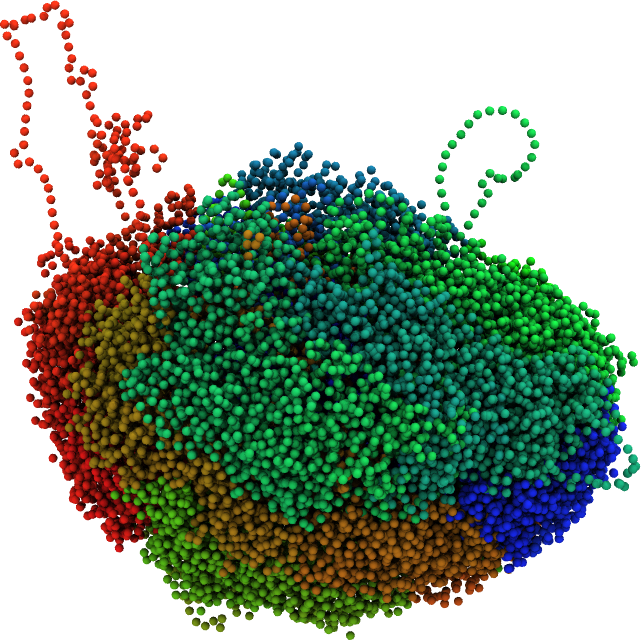
\includegraphics[height=\cellrenderingheight]{cell1_frame104_scene1.png}
  \caption{Cell 1, frame 104, scene 1}
  \label{img:cell1_frame104_scene1}
\end{figure}

\begin{figure}[H]
\centering
  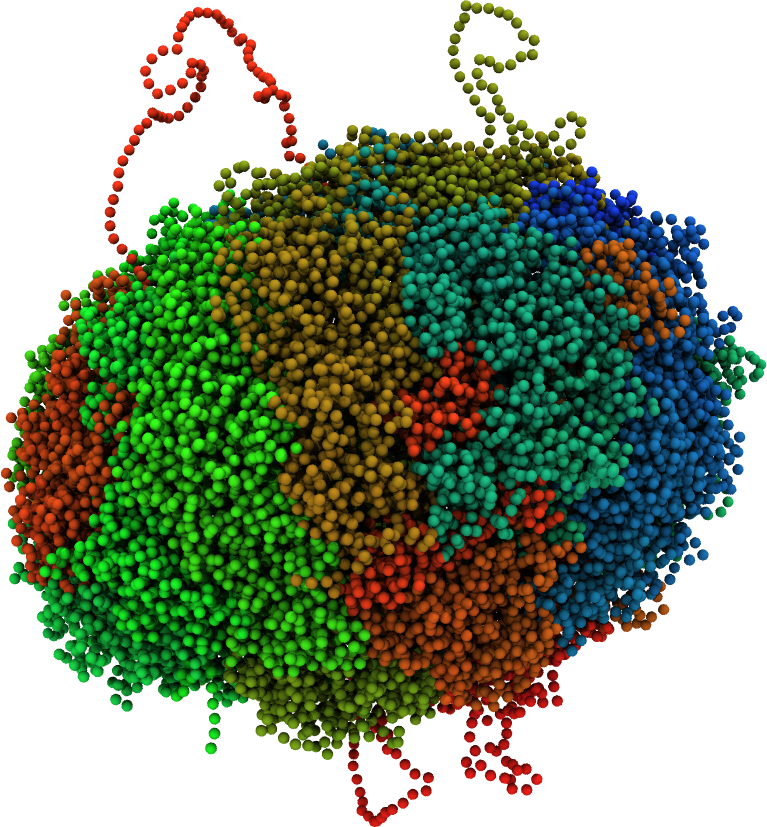
\includegraphics[height=\cellrenderingheight]{cell2_frame104_scene1.png}
  \caption{Cell 2, frame 104, scene 1}
  \label{img:cell2_frame104_scene1}
\end{figure}

\begin{figure}[H]
\centering
  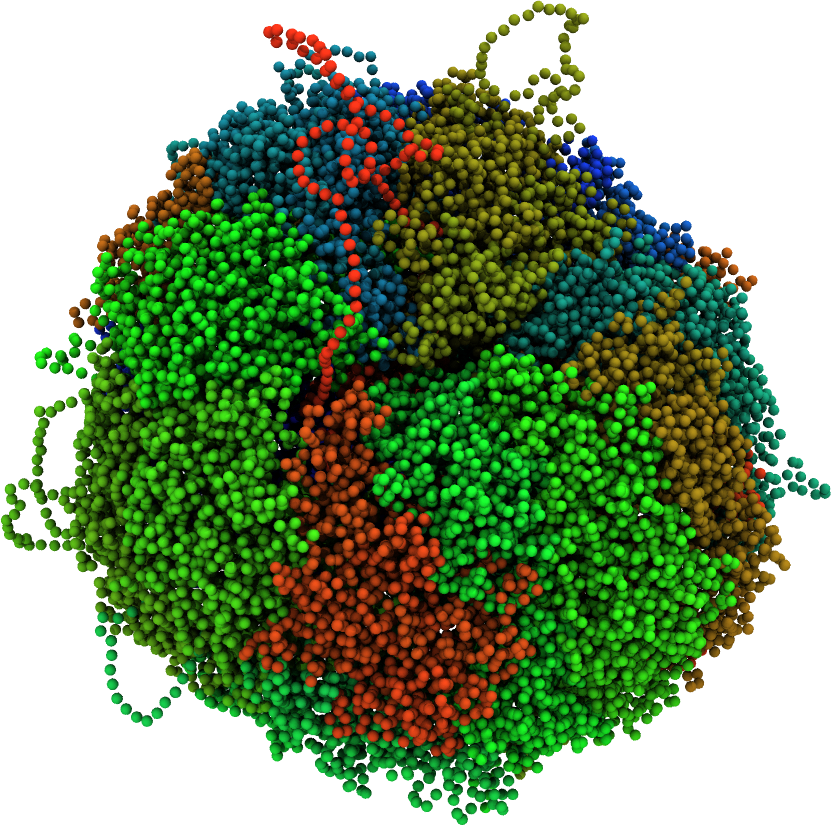
\includegraphics[height=\cellrenderingheight]{cell2_frame104_scene2.png}
  \caption{Cell 2, frame 104, scene 2}
  \label{img:cell2_frame104_scene2}
\end{figure}

\begin{figure}[H]
\centering
  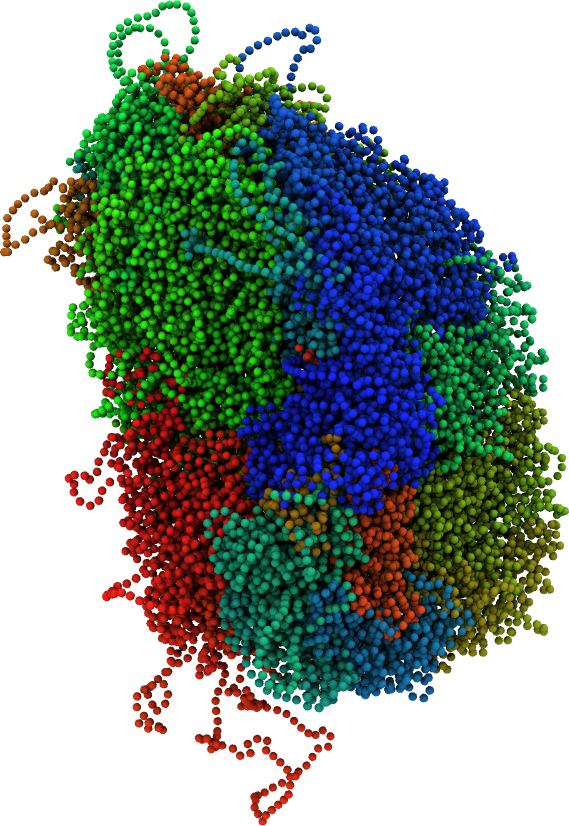
\includegraphics[height=\cellrenderingheight]{cell3_frame104_scene1.png}
  \caption{Cell 3, frame 104, scene 1}
  \label{img:cell3_frame104_scene1}
\end{figure}

\begin{figure}[H]
\centering
  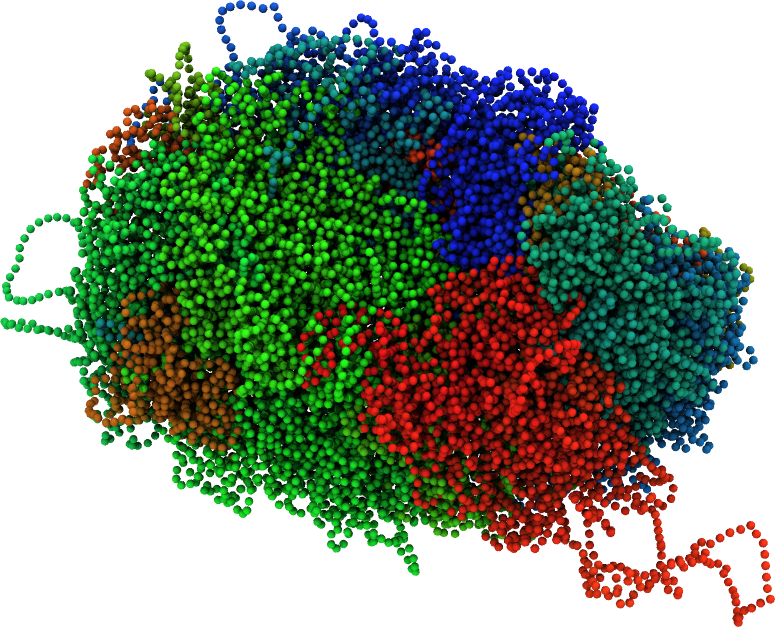
\includegraphics[height=\cellrenderingheight]{cell3_frame104_scene4.png}
  \caption{Cell 3, frame 104, scene 4}
  \label{img:cell3_frame104_scene4}
\end{figure}

\begin{figure}[H]
\centering
  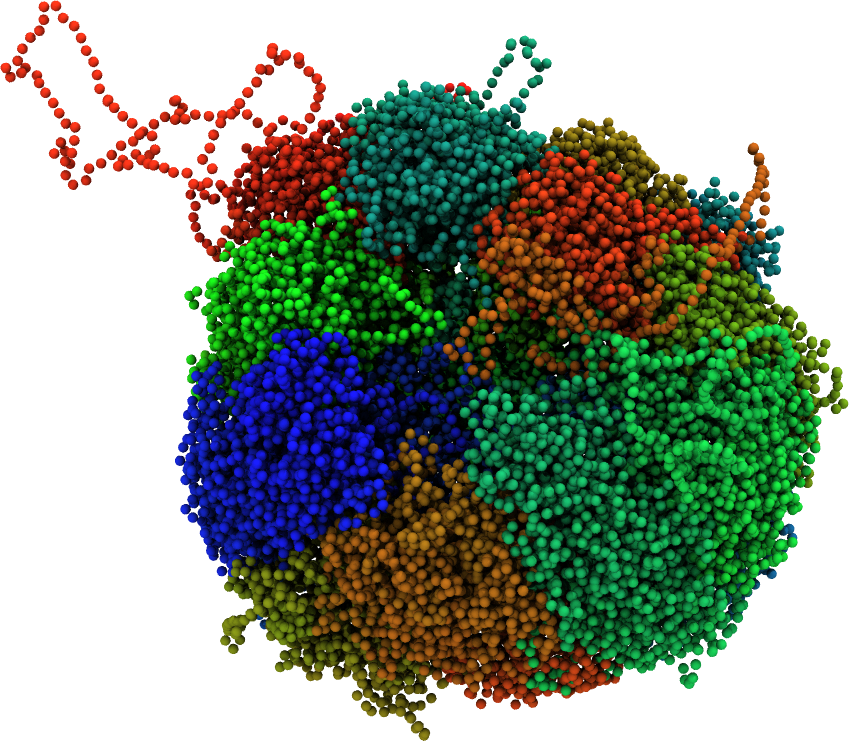
\includegraphics[height=\cellrenderingheight]{cell4_frame104_scene1.png}
  \caption{Cell 4, frame 104, scene 1}
  \label{img:cell4_frame104_scene1}
\end{figure}

\begin{figure}[H]
\centering
  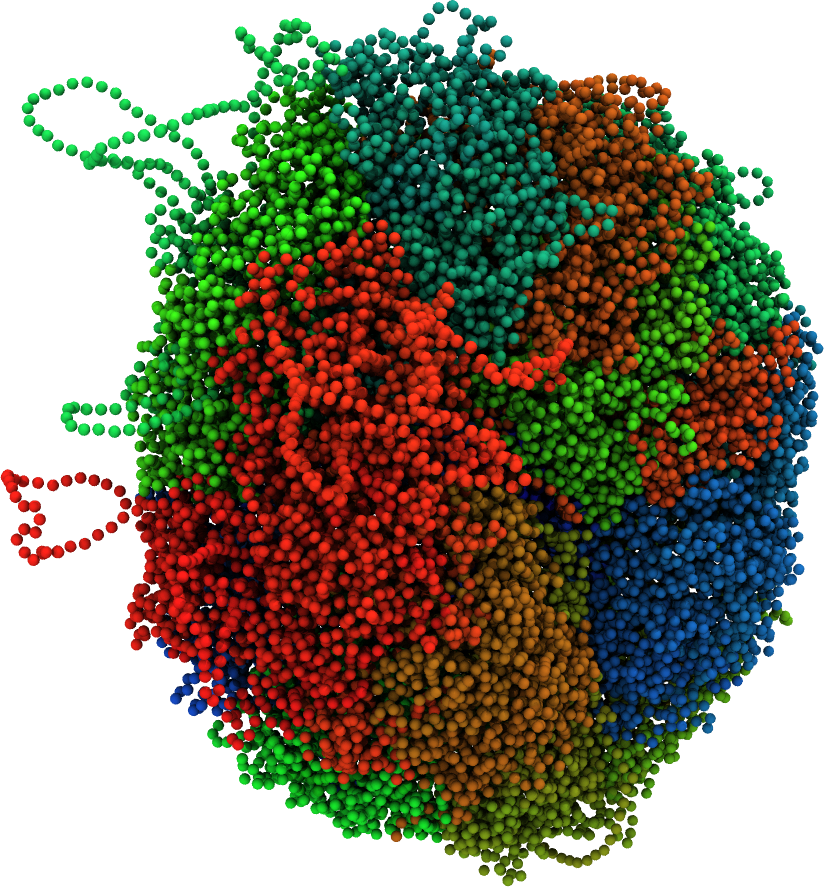
\includegraphics[height=\cellrenderingheight]{cell5_frame036_scene1.png}
  \caption{Cell 5, frame 36, scene 1}
  \label{img:cell5_frame036_scene1}
\end{figure}

\begin{figure}[H]
\centering
  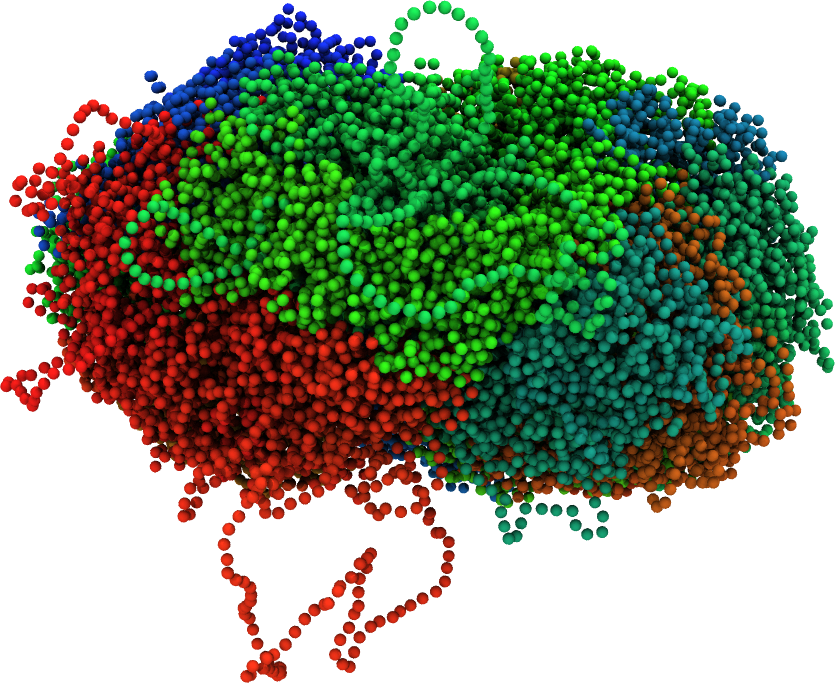
\includegraphics[height=\cellrenderingheight]{cell5_frame036_scene2.png}
  \caption{Cell 5, frame 36, scene 2}
  \label{img:cell5_frame036_scene2}
\end{figure}

\begin{figure}[H]
\centering
  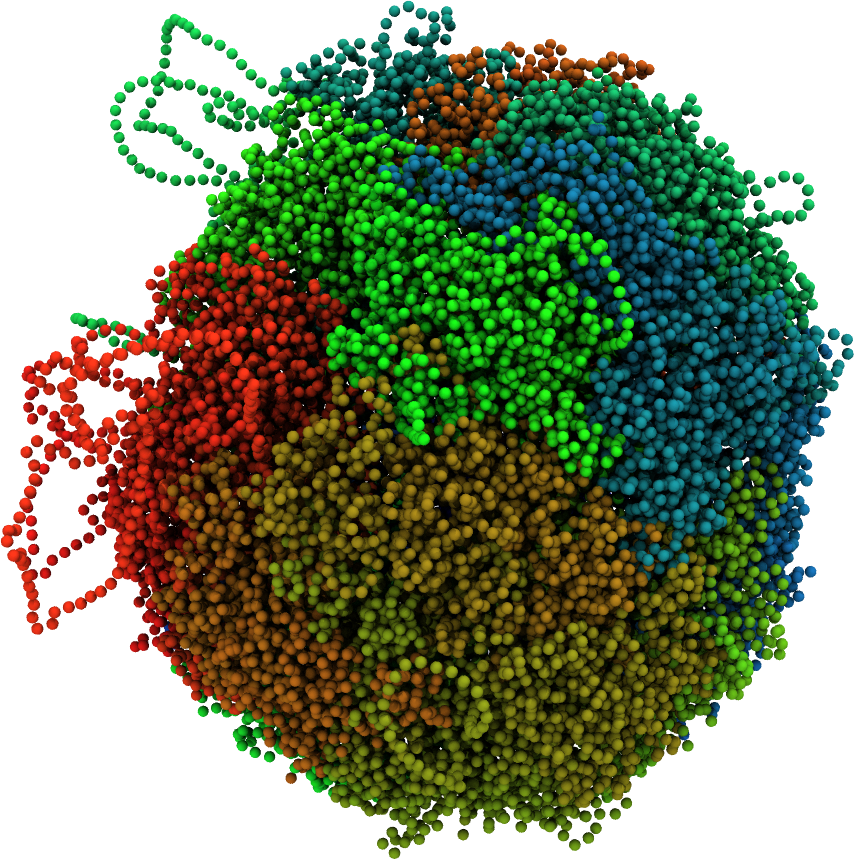
\includegraphics[height=\cellrenderingheight]{cell5_frame104_scene1.png}
  \caption{Cell 5, frame 104, scene 1}
  \label{img:cell5_frame104_scene1}
\end{figure}

\begin{figure}[H]
\centering
  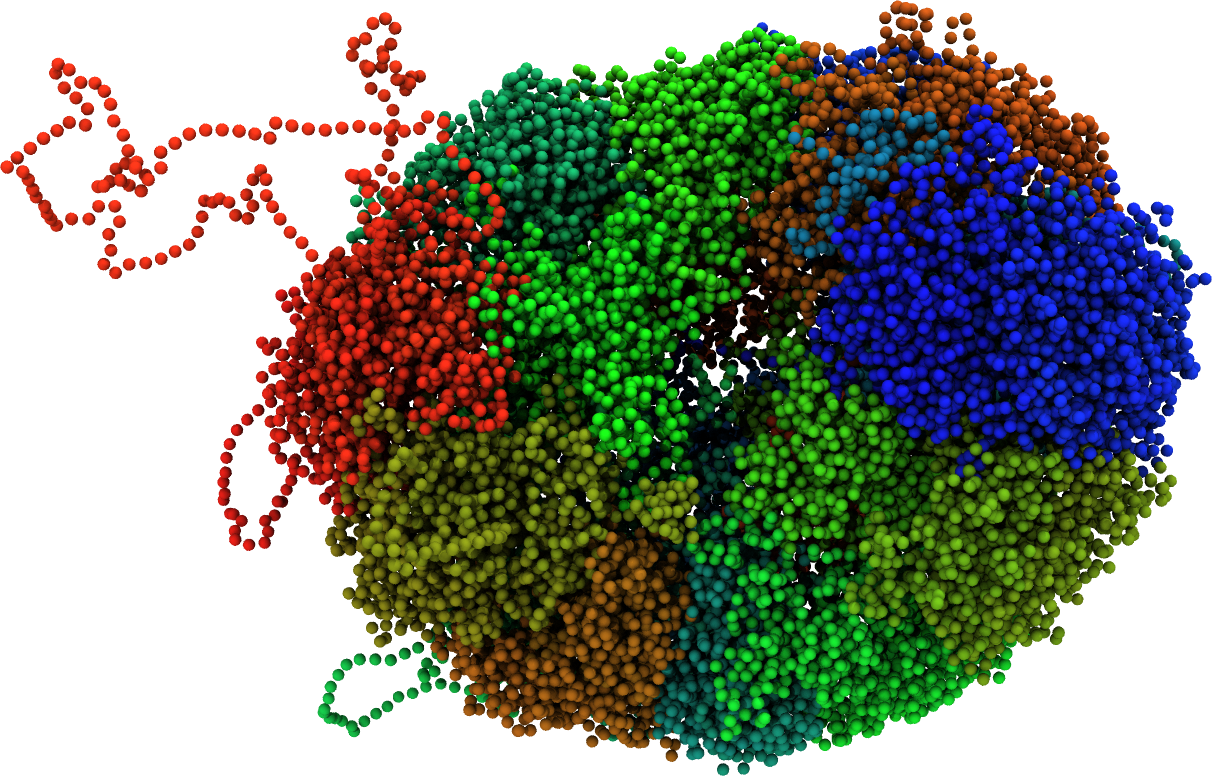
\includegraphics[height=\cellrenderingheight]{cell6_frame104_scene1.png}
  \caption{Cell 6, frame 104, scene 1}
  \label{img:cell6_frame104_scene1}
\end{figure}

\begin{figure}[H]
\centering
  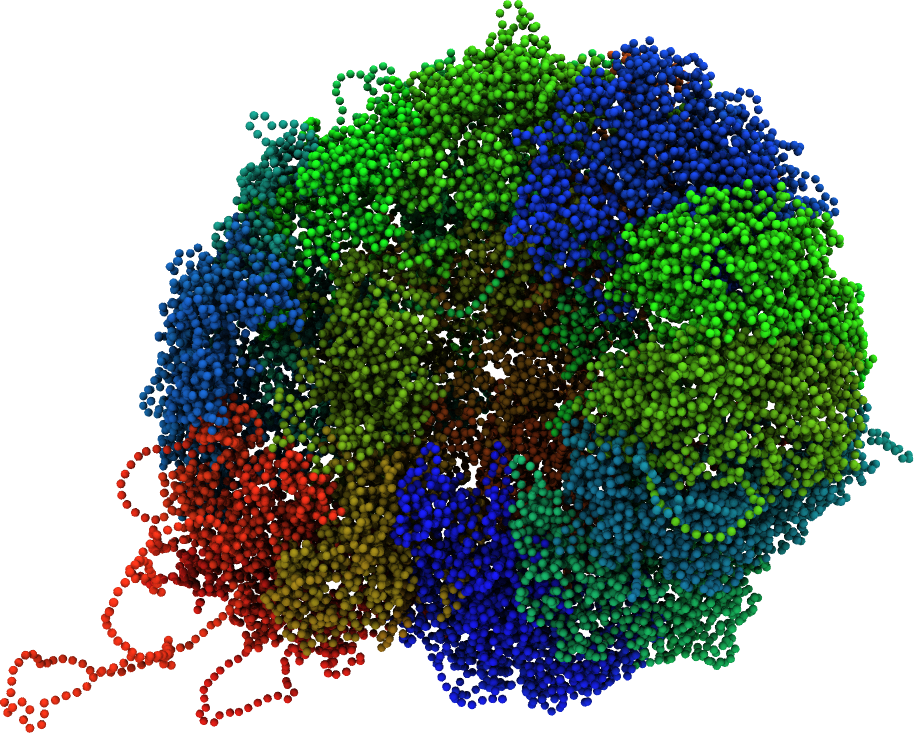
\includegraphics[height=\cellrenderingheight]{cell7_frame104_scene1.png}
  \caption{Cell 7, frame 104, scene 1}
  \label{img:cell7_frame104_scene1}
\end{figure}

\begin{figure}[H]
\centering
  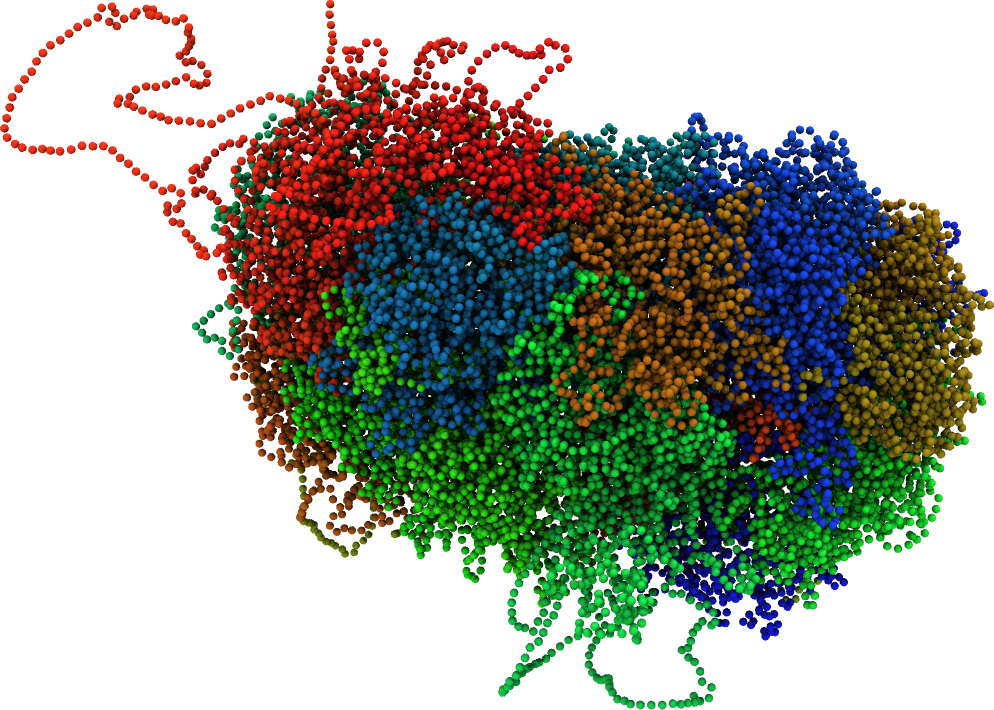
\includegraphics[height=\cellrenderingheight]{cell8_frame104_scene2.png}
  \caption{Cell 8, frame 104, scene 2}
  \label{img:cell8_frame104_scene2}
\end{figure}


% chapter renderings_of_simuated_cells (end)

\chapter{Used Software} % (fold)
\label{cha:used_software}

Figures were created using matplotlib\cite{j_d_hunter_matplotlib_2007} and seaborn\cite{waskom_seaborn_2021}.

\begin{table}[H]
\centering
\label{tab:used_software}
\caption{Software used for simulation and data analysis. Two systems were used, the top one a Manjaro Linux (based on Arch Linux) system and the bottom one a Microsoft Windows system with Anaconda}
  \begin{tabular}{c @{\phantom{abc}} c @{\phantom{abc}} c}
  \toprule
    Package & Version & Package Source \\
  \midrule
    HOOMD-blue & 1.9.7 & built from source \\
    numpy &  & arch repo \\
    scipy &  & arch repo \\
    pandas &  & arch repo \\
    matplotlib &  & arch repo \\
    gsd & & \\
    vmd & & \\
  \midrule
    numpy & 1.20.3 & anaconda \\
    scipy & 1.7.1 & anaconda \\
    pandas & 1.3.4 & anaconda \\
    matplotlib & 3.4.3 & anaconda \\
    gsd & 2.5.1 & pip \\
    hicreppy & 771cf72 & github \\
  \bottomrule
  \end{tabular}
\end{table}

\todo{packages and versions for linux system}


% chapter used_software (end)

%_______________________________________________________________________________
\chapter{Weiterführende Details zur Arbeit} % (fold)
\label{cha:weiterführende_details_zur_arbeit}

Manch wichtiger Teil Ihrer tatsächlichen Arbeit ist zu technisch 
und würde den Hauptteil des Textes unübersichtlich machen, 
beispielsweise wenn es um die Details des Versuchsaufbaus in einer 
experimentellen Arbeit oder um den für eine numerische Auswertung 
verwendeten Algorithmus geht. Dennoch ist es sinnvoll, entsprechende 
Beschreibungen in einem Anhang Ihrer Bachelorarbeit aufzunehmen. 
Insbesondere für zukünftige Arbeiten, die an Ihre Bachelorarbeit 
anschließen, sind dies manchmal hilfreiche Informationen.

% chapter weiterführende_details_zur_arbeit (end)

%_______________________________________________________________________________
\chapter{Thanking} % (fold)
\label{cha:thanking}

... an wen auch immer. Denken Sie an Ihre Freundinnen und Freunde, 
Familie, Lehrer, Berater und Kollegen.

% chapter thanking (end)

%_______________________________________________________________________________
% \chapter{References} % (fold)
% \label{cha:references}

% Machen Sie genaue Angaben, so dass die verwendeten Literaturstellen 
% eindeutig identifiziert und aufgefunden werden können.
% Bei Lehrbüchern cite{Weinberg:1995mt} ist es sinnvoll, 
% den Titel anzugeben, eventuell auch die Ausgabe. Bei Artikeln in 
% Fachzeitschriften cite{Moch:2001zr} ist es üblich, nur die 
% gebräuchlichen Abkürzungen für den Titel der Zeitschrift, Band, 
% Erscheinungsjahr und Seite anzugeben. Unter Umständen kann es auch 
% sinnvoll sein, im Internet aufgefundene Informationsquellen anzugeben, 
% zum Beispiel für Software cite{LoopTools} oder zu den Details von 
% Ergebnissen großer experimenteller Kollaborationen. Es ist 
% selbstverständlich, dass Sie auch Bachelor- cite{BA:Freund}, 
% Diplom- oder Doktorarbeiten angeben, wenn Sie diese in Ihrer eigenen 
% Arbeit verwendet haben.
% \medskip

% Im folgenden Beispiel werden die in der Datei \texttt{h-physrev3.bst} 
% enthaltenen Anweisungen als Stilvorlage verwendet. Andere 
% Möglichkeiten für die Gestaltung eines Literaturverzeichnisses 
% findet man im Internet: \url{http://janeden.net/bibliographien-mit-latex}.

% \renewcommand{\bibname}{Literaturverzeichnis} 
% \bibliographystyle{h-physrev3}
% \begin{thebibliography}{99}

% %\cite{thepnews}
% \bibitem{EbelBliefert}
% H.\ F.\ Ebel, C.\ Bliefert, 
%   ``Bachelor-, Master- und Doktorarbeit: Anleitungen für den 
%   naturwissenschaftlich-technischen Nachwuchs,''
%   Wiley-VCH, Weinheim (2009). 
% \bibitem{thepnews}
%   S.~Becker, D.~Götz, C.~Reuschle, C.~Schwan, S.~Weinzierl,  
%   \url{http://wwwthep.physik.uni-mainz.de/site/news/168/}.

% %\cite{Weinberg:1995mt}
% \bibitem{Weinberg:1995mt}
%   S.~Weinberg,
%   ``The Quantum theory of fields. Vol. 1: Foundations,''
%   Cambridge, UK: Univ. Pr. (1995) 609 p.

% %\cite{Moch:2001zr}
% \bibitem{Moch:2001zr}
%   S.~Moch, P.~Uwer, S.~Weinzierl,
%   %``Nested sums, expansion of transcendental functions and multiscale 
%   % multiloop integrals,''
%   J.\ Math.\ Phys.\  {43 } (2002)  3363-3386.
%   [hep-ph/0110083].

% %\cite{LoopTools}
% \bibitem{LoopTools}
%   T.~Hahn, 
%   ``The LoopTools Site,''
%   \url{http://www.feynarts.de/looptools/}.

% %\cite{BA:Freund}
% \bibitem{BA:Freund}
%   B.~Freund, 
%   Bachelorarbeit, Johannes Gutenberg-Universität Mainz, 2012.

% \end{thebibliography}

% chapter references (end)


\end{document}